\documentclass[../main-v1.tex]{subfiles}
\begin{document}

\chapter{Data and Processing Volume Estimates \hideme{Schellman, Junk, Muether - started numbers and figures need updating}}
\label{ch:est}
\fixme{Heidi: moved tables of numbers from intro to here.  Still needs better organization}
%anne In this chapter we will 
This chapter describes the assumptions that go into a bottoms-up estimate of data volumes and describe possible methods of reducing the total volumes while retaining physics capabilities. 

\section{Introduction \hideme{Schellman - need a paragraph}}


\section{Assumptions \hideme{Schellman - draft}}
\label{sec:est:assume}  %% fix label according to section

\subsection{Raw Data Assumptions \hideme{Schellman - draft}}
DUNE's detectors will produce information from a variety of technologies.  We anticipate that raw data volumes will be dominated by the digitized waveforms from \dword{lar} detectors, and to a lesser extent \dwords{pd}, in the prototype runs at the \dword{cern}, the \dword{fd}, and the \dword{nd}.  
%anneThese raw data volumes can be reduced by the \dword{daq} system by several means.
The \dword{daq} system can reduce these raw data volumes by several means, i.e.,
\begin{itemize} 
\item triggered readout of particular time slices,
\item triggered readout of particular geographic regions,
\item lossless zero suppression,
\item lossy zero suppression, and
\item hardware pattern recognition.
\end{itemize}

Overall, we assume that the above methods can reduce data volumes from the hundreds of exabytes that would be produced by continuous readout to a manageable 30\,PB/year. 

\subsection{Derived Data Assumptions \hideme{Schellman - draft}}

 \begin{dunetable}[Data Retention Policies]{llrrrr}{tab:est:retention}
{Retention policies by data tier}
Tier&Description&Tape copies& Lifetime &Disk Copies& Lifetime\\ \toprowrule
Raw & Physics data& 2 & indefinitely & 1 & 1 year\\ \colhline
Test & test and commissioning & 1 &6 months &1 & 6 months \\ \colhline
Hits & reconstructed hits & 1 & 10 years & 1 & 1 month \\ \colhline
Reco & pattern recognition &1 & 10 years & 2 & 2 years\\
\end{dunetable}

\section{ProtoDUNE \hideme{Schellman - draft}}
\label{sec:est:ProtoDUNE}  

Our estimates  are largely based on our experience with the %anne single and dual-phase 
\dword{sp} and \dword{dp} prototype detectors that ran at the \dword{cern} in late 2018. \todo{(anne) they operated at different times; DP was later} The \dword{pdsp} detector used \dword{hd} \dword{tpc} technology, read out by six \dwords{apa} and a mix of \dwords{pd}. The corresponding first \dword{fd} module will have 150 \dwords{apa} and \dwords{pd} based on the \dword{arapuca} technology. The second \dword{fd} module will have \dword{sp} vertical drift readout but will share technology with %anne the dual-phase prototype. 
\dword{pddp}. Data rates and assumptions for \dword{protodune} have been documented in \todo{move doc to publicly-accessible place then add to bib \href{docdb:20515}{https://docs.dunescience.org/cgi-bin/private/ShowDocument?docid=20515}. } Table~\ref{tab:est:usefulpd} provides useful quantities for data volumes derived from the \dword{pdsp} experience. 

 \begin{dunetable}[Useful quantities for computing far detector data volumes]{lrr}{tab:est:usefulpd}
{Useful quantities for computing estimates for \dword{hd}
readout based on \dword{pdsp} experience.  }%\rowtitlestyle
Quantity&Value&Explanation\\
\toprowrule
%{\bf Far Detector Beam:}\\ \colhline
Number of channels/APA&2,560&\\
Readout time & 3 ms&\\
\# of time slices & 6000&\\
Single APA readout &23 MB& Uncompressed  estimate\\ \colhline
APAs & 6 &\\
Full detector readout &178 MB& Uncompressed real \\ \colhline
Full detector readout &71 MB& Compressed real \\ \colhline
Effective compression factor &2.5&\\ \colhline
Beam rep. rate&4.5 Hz&Average\\ \colhline
Hit reconstruction time CPU time/APA& 30 sec&from MC/ProtoDUNE\\ \colhline
Pattern recognition time CPU time event & 400 sec&from MC/ProtoDUNE\\ \colhline
Simulation time CPU time event & 2700 sec&from MC/ProtoDUNE\\ \colhline
Memory footprint/APA&0.5-1GB&ProtoDUNE experience\\ 
\end{dunetable}

 

For example, uncompressed \dword{sp} data from \dword{pdsp} were observed to be around 178\,MB in size, which is the amount expected for the number  of \dword{tpc} channels read + a 20\% overhead for other detectors and headers.  Compressed \dword{sp} data averages 71\,MB, consistent with compression by a factor of 2.5.  

%anne Dual phase data 
\dword{pddp} read out two \dword{crp} units for the 2019 run.  Observed data size without compression  was 110\,MB.  %Numbers for 2018 and 2019 have been 

In fall 2021, single-phase vertical drift readout has been tested in a smaller \coldbox with full \dword{protodune} tests of both \dword{hd} and \dword{vd} technology with beam and cosmic rays slated for 2022-24. Data volume estimates include data and simulation for this second prototype test campaign. 

% For the far detector with APA's we assume 

% \section{ProtoDUNE II VD and HD discussion \hideme{Schellman/Kirby/Pennacchio - needed}}




% [DUNE-doc-20515-v9]

\section{Far Detector Data Volume Estimates \hideme{Schellman - draft}}
\label{sec:est:FD}  

\subsection{Horizontal Drift}
For \dword{hd} \dword{fd} data volumes, we use our \dword{pdsp} experience and assume that raw data sizes and hit-finding CPU times scale with the number of \dwords{apa}, while pattern recognition and simulation times scale with the number of interactions. 

 \begin{dunetable}[Useful quantities for computing \dshort{hd} data volume
estimates]{lrr}{tab:est:usefulfd}
{Useful quantities for computing estimates for \dword{hd}
readout.}%\rowtitlestyle
Quantity&Value&Explanation\\
\toprowrule
{\bf Far Detector Beam:}\\ \colhline
Single APA readout &41.5 MB& Uncompressed 5.4 ms\\ \colhline
APAs per module& 150&\\
Compression factor &2.5 &\\
One full module readout &6.22  GB& Uncompressed 5.4 ms\\ \colhline
One full module readout &2.49  GB& Compressed 5.4 ms\\ \colhline
Beam rep. rate&\beamreprate&Untriggered\\ \colhline
Hit finding CPU time/APA&30 sec&from MC/ProtoDUNE\\ \colhline
Pattern recognition CPU time/event&400 sec&from MC/ProtoDUNE\\ \colhline
Simulation time CPU time event & 2700 sec&from MC/ProtoDUNE\\ \colhline
Memory footprint/APA&0.5-1GB&ProtoDUNE experience\\ \colhline
{\bf Supernova:}\\ \colhline
Single channel readout &300 MB& Uncompressed 100 s\\ \colhline
Four module readout& 460 TB& Uncompressed 100 s\\ \colhline
Four module readout& 184 TB& Compressed 100 s\\ \colhline
Trigger rate&1  per month&(assumption)\\
\end{dunetable}


DUNE \todo{make public, then bib \href{docdb:14893}{https://docs.dunescience.org/cgi-bin/private/ShowDocument?docid=14983}} describes the expected event rates for various signatures in a \dword{fd} module.  These can be combined with the above numbers to provide  the integrated data estimates shown in Table~\ref{tab:est:hdfdrates}. 

 \begin{dunetable}
 [Horizontal Drift data volumes] {|l |r r r |}{tab:est:hdfdrates}
{Data sizes and rates for different processes in each horizontal drift detector module.  Uncompressed data sizes are given. As readouts will be self-triggering an extended 2.6 ms readout window is used instead of the 3ms for the triggered \dword{pdsp} runs.  We assume beam uptime of 50\% and 100\% uptime for non-beam science. These numbers are derived from references \cite{bib:docdb16028} and \cite{bib:docdb14983}.}
%\rowtitlestyle
%Quantity&Value&Explanation\\
%\toprowrule
%\begin{tabular}{|l |r r r |}
%\hline
Process & Rate/module & \qquad size/instance &\qquad  size/module/year\\
\toprowrule
Beam event & 41/day & 3.8 GB&30 TB/year\\
Cosmic rays &4,500/day&  3.8 GB& 6.2 PB/year\\
Supernova trigger& 1/month& 140 TB& 1.7 PB/year\\
Calibrations&2/year&750 TB& 1.5 PB/year\\
\colhline 
Total& & &9.4 PB/year\\
\end{dunetable}%

\subsection{Far Detector Module with Vertical Drift Readout}

 Table~\ref{tab:est:vdfdrates} summarizes expected data rates and volumes from physics signals of interest in % anne a Far Detector based on Vertical drift technology.
 \dword{spvd}. % Anne: this dword doesn't quite work...
 The data volume  corresponding  to calibration events can be considered to be similar to the one assumed in Table~\ref{tab:est:hdfdrates}; a more detailed estimation is ongoing. 
 
 \begin{dunetable}
 [%anneVertical Drift Far detector 
 \dshort{spvd} data volumes] {|l |r r r |}{tab:est:vdfdrates}
{Data sizes and rates for different processes in \dword{spvd}. %anne a far detector module based on vertical drift technology. 
Uncompressed data sizes are given. As readouts will be self-triggering, an extended 4.25\,ms readout window is used.  We assume beam uptime of 50\% and 100\% uptime for non-beam science~\cite{bib:docdb16028,bib:docdb14983}.  %anne These numbers are derived from references~\cite{bib:docdb16028} and~\cite{bib:docdb14983}.
} 
Process & Rate/module & \qquad event size  &\qquad  size/module/year\\
\hline
Beam event & 41/day & 8 GB& 63 TB/year\\
Cosmic rays &4,500/day&  8 GB& 12.5 PB/year\\
Supernova trigger& 1/month& 130 TB& 2 PB/year\\
Calibrations&2/year& & 1.5 PB/year\\
\hline 
Total& & &16 PB/year\\
\end{dunetable}% 
\todo{will have to fix all docdb references -no dune docdb docs are accessible to the public now}
%The \dword{vd} numbers are computed assuming a  full module readout for a time window equals to 2.2 the the drift window. 

\subsection{Far Detector Summary}
Overall, bottoms-up estimates yield data volumes of around 9.4 and 16\,PB/year/module.  Lossless compression and restriction of the readout to geographical regions of interest should reduce this volume substantially. However, additional modules will  increase these rates.  A maximum rate of 30\,PB/year across all modules and modes of operation has been specified.  We will note that 30\,PB/year is  an average of 1.3\,GB/sec, less than the rates already demonstrated for \dword{protodune} %acquisition 
\dword{daq} and storage.  In principle, at 2.5\,CPU-sec/MB of compressed input, a few thousand cores could keep up with these data rates,  but this throughput must be maintained over many years.   In addition, \dword{snb} candidates may require bursts of  much higher \dword{daq} and processing rates. %Table \ref{tab:exec-comp-bigpicture-es} summarizes the computational characteristics expected for \dword{fd} data. 


\section{Near Detector Data Volumes \hideme{Schellman/Muether - needs significant update}}
\label{sec:est:ND}  
\todo{Muether/Junk - Need to update these numbers}
This section is based on the estimates provided in the near detector (\dword{nd}) \dword{cdr}~\cite{DUNE:2021tad}. % \hideme{Add ND CDR citation}

Table~\ref{tab:nd_data_volume_estimates} summarizes the expected data sizes from the \dword{nd}. Due to the much higher data density in the near detector, CPU times/beam spill are expected to be much higher and are estimated to be 300\,CPU/sec/spill using current processors for $1.5\times 10^7$ spills/year. Simulated data samples will need to be an order of magnitude larger and thus require at least 10 times the CPU power.  This leads to a rough estimate of CPU needed for \dword{nd} reconstruction and simulation of approximately 3,000 core-years/year.

\begin{dunetable}[Near Detector Data Estimates]
{l r}
{tab:nd_data_volume_estimates}
{Annual DUNE near detector data volume estimates.  No compression is assumed.}
Type & Volume/year\\ \toprowrule
    {\bf \dword{ndlar}}     &  \\
    \quad\quad In-spill data & 144 TB \\
    \quad\quad Out-of-spill cosmics & 16 TB\\
    \quad\quad Calibration & 16 TB\\
    \quad\quad Total & 176 TB \\\toprowrule
    {\bf \dword{ndgar}}           & \\
    \quad\quad In-spill data & 52 TB \\
    \quad\quad Out-of-spill cosmics & 10 TB \\
    \quad\quad Calibration & 6 TB\\
    \quad\quad Total & 68 TB \\\toprowrule
    {\bf \dword{sand}}        & \\
        \quad\quad In-spill data & 4 TB\\
    \quad\quad Out-of-spill cosmics & 1 TB\\
    \quad\quad Calibration & 1 TB \\
    \quad\quad Total & 6 TB \\\toprowrule
    {\bf Total ND} & {\bf 250 TB}\\
\end{dunetable}

\begin{dunetable}
[CPU estimates for Near Detector]
{l r}
{tab:NDCPUPerEvent}
{Preliminary CPU estimates per event for the DUNE near detector components, in seconds.}
Type&time/event\\ \toprowrule
    {\bf LArTPC} &  \\
    \quad\quad Monte Carlo gen+sim & 100 s \\
    \quad\quad Reconstruction & 60 s\\\toprowrule
  {\bf MPD} &  \\
    \quad\quad Monte Carlo gen+sim & 100 s\\
    \quad\quad Reconstruction & 12 s\\\toprowrule
    {\bf SAND} & \\
    \quad\quad Monte Carlo gen+sim & 100 s\\
    \quad\quad Reconstruction & 10 s\\
\end{dunetable}

\section{Summary \hideme{Schellman - needs update}}
\label{sec:est:volumes}

Given the above estimates we can  estimate total disk and CPU needs every year.  The September 2021 version of these numbers is documented in~\cite{bib:docdb23419}

Figure~\ref{fig:est:events} shows the assumed number of events/year for each detector type.  

\begin{dunefigure}
[Event estimates]
{fig:est:events}
{Number of events per year used in data volume estimates. Left is through 2030, right is the same through 2040.  }
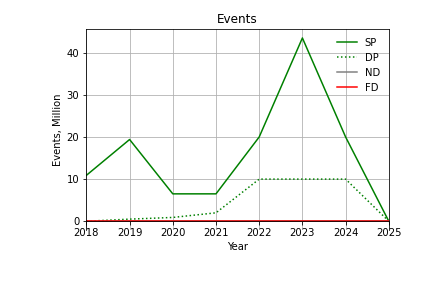
\includegraphics[width=0.49\textwidth]{graphics/IntroFigures/soon/Events.png}
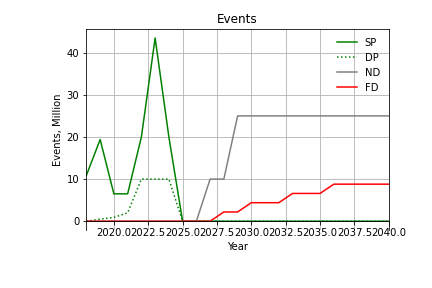
\includegraphics[width=0.49\textwidth]{graphics/IntroFigures/2040/Events.png}
\end{dunefigure}

CPU and size/readout are drawn from the above estimates. We then make the following assumptions about data sizes and retention.  

\begin{itemize}
\item Two copies of raw data are retained indefinitely.
\item Commissioning data is marked test and one copy is retained on disk for six months. 
\item Reconstruction is performed on the full data sample once/year and two copies are retained on disk for two years.  
\item Analysis includes calibration and is  equivalent in CPU utilization to reconstruction but produces smaller outputs. 
\end{itemize}

Figures~\ref{fig:est:disk}, \ref{fig:est:tape}, and~\ref{fig:est:cores} illustrate the estimated storage and CPU needs through 2026 and 2040.  In the early years, \dword{pd} and \dword{nd} prototype tests dominate while commissioning and operation of the first (and second) \dword{fd} module(s) and the \dword{nd} become important after 2026. 

\begin{dunefigure}
[Disk estimates]
{fig:est:disk}
{Estimated size of various samples in PB. This estimate includes retention policies and multiple copies.}
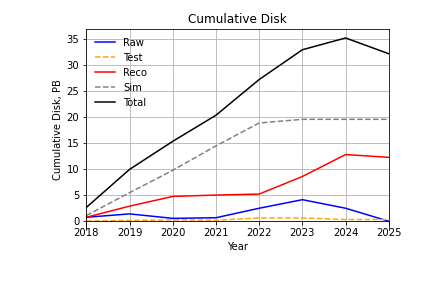
\includegraphics[width=0.49\textwidth]{graphics/IntroFigures/soon/Cumulative-Disk.png}
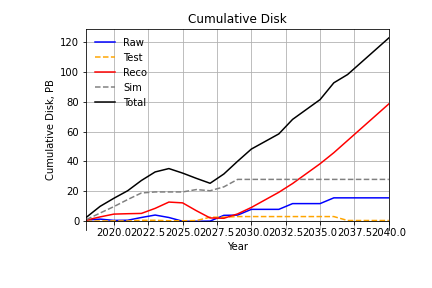
\includegraphics[width=0.49\textwidth]{graphics/IntroFigures/2040/Cumulative-Disk.png}
\end{dunefigure}

\begin{dunefigure}
[Tape estimates]
{fig:est:tape}
{Estimated size of various samples in PB. This estimate includes retention policies and multiple copies.}
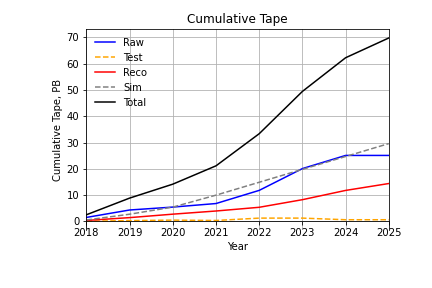
\includegraphics[width=0.49\textwidth]{graphics/IntroFigures/soon/Cumulative-Tape.png}
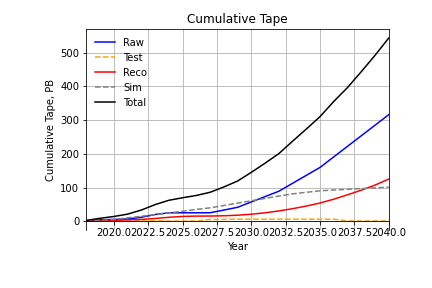
\includegraphics[width=0.49\textwidth]{graphics/IntroFigures/2040/Cumulative-Tape.png}

\end{dunefigure}

\begin{dunefigure}
[Tape estimates]
{fig:est:cores}
{Estimated CPU needs for  various samples.  The units are present day cores assuming 70\% efficiency.}
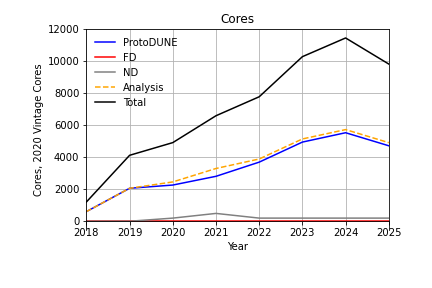
\includegraphics[width=0.49\textwidth]{graphics/IntroFigures/soon/Cores.png}
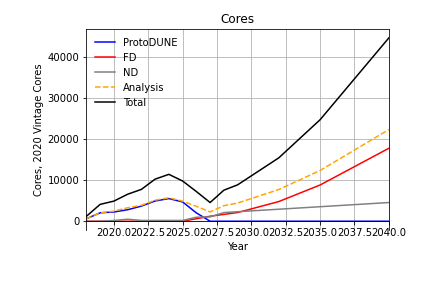
\includegraphics[width=0.49\textwidth]{graphics/IntroFigures/2040/Cores.png}
\end{dunefigure}


\end{document}